\problemset{Теория вероятностей и математическая статистика}
\problemset{Индивидуальное домашнее задание №3}

% Команда ниже задает "название" или слово, которое будет
% отображаться вместо proof или "доказательство"
% поскольку у нас в ИДЗ задачи - то нужно слово "Решение"
\renewcommand*{\proofname}{Решение}

Случайный вектор $(\xi,\eta)$ имеет равномерное распределение в области $D$:
\[
D = \{(x,y)\text{ }|\text{ }2x - y \ge 0, x \le 0, y \ge -2\}
\]
$\zeta = 3\xi^4 + 2$, $\nu = \lfloor 5\eta\rfloor$, $\mu = -4\xi + 2\eta$

%%%%%%%%%%%%%% ЗАДАНИЕ №1 %%%%%%%%%%%%%%
%% Условие задания №1
\begin{problem}
Найти $p_{\xi,\eta}(x,y)$, функции и плотности распределения компонент. Построить графики функций распределений $F_{\xi}(x)$ и $F_{\eta}(y)$. Будут ли компоненты независимыми?
\end{problem}

%% Решение задания №1
\begin{proof}
Случайный вектор имеет равномерное распределение в области D, значит что:
\[
p_{\xi,\eta}(x,y) = \begin{cases}
    C, & (x,y) \in D\\
    0, & \text{в отс. сл.}
    \end{cases}
\]
\begin{figure}[h!]
    \centering
    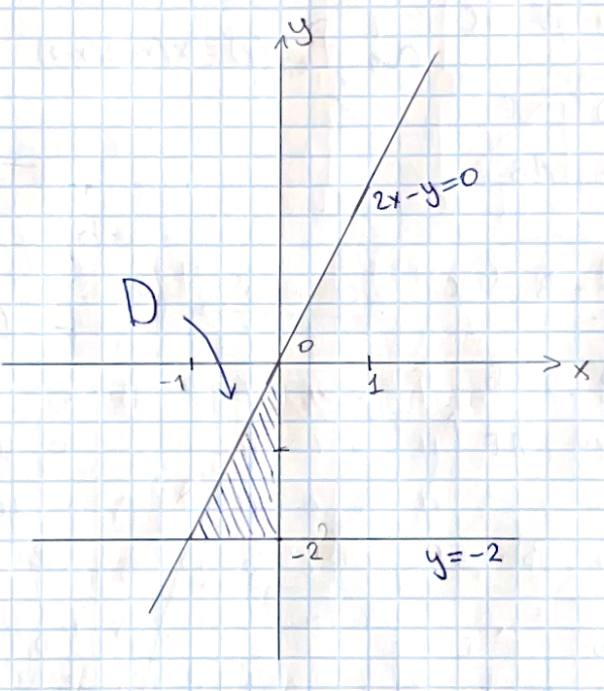
\includegraphics[width=0.5\linewidth]{1.jpeg}
    \caption{}
    \label{fig:enter-label}
\end{figure}
Изобразим область $D$ (см. рис. 1). По свойству имеем, что $ \iint_{\Real^2}p_{\xi,\eta}(x,y)dxdy = 1$:
\[
\iint_{\Real^2}p_{\xi,\eta}(x,y)dxdy = \iint_{D}p_{\xi,\eta}(x,y)dxdy = \int_{-1}^{0}dx\int_{-2}^{2x}Cdy = C = 1 \Rightarrow C = 1
\]
Итого:
\[
p_{\xi,\eta}(x,y) = \begin{cases}
    1, & (x,y) \in D\\
    0, & \text{в отс. сл.}
    \end{cases}
\]
Найдем плотности распределения компонент.\\
Для компоненты $\xi$:
\begin{gather*}
\int_{\Real}p_{\xi,\eta}(x,y)dy = \int_{-2}^{2x}dy = 2x + 2\\
p_{\xi}(x) = \begin{cases}
    2x + 2, & x \in [-1;0]\\
    0, & \text{в отс. сл.}
    \end{cases}
\end{gather*}
Для компоненты $\eta$:
\begin{gather*}
\int_{\Real}p_{\xi,\eta}(x,y)dx = \int_{y/2}^{0}dx = -\frac{y}{2}\\
p_{\eta}(x) = \begin{cases}
    -\frac{y}{2}, & y \in [-2;0]\\
    0, & \text{в отс. сл.}
    \end{cases}
\end{gather*}
Проверим компоненты на независимость. Должно выполняться условие $p_{\xi,\eta}(x,y) = p_{\xi}(x)\cdot p_{\eta}(y)$ во всех точках.
\[
1 = -\frac{y}{2}\cdot(2x + 2)\\
\]
Рассмотрим точку (0,0):
\[
1 = -\frac{0}{2}\cdot(2\cdot 0 + 2) = 0 - \text{неверно}\Rightarrow\text{компоненты зависимы}
\]
Найдем функции распределений$F_{\xi}(x)$ и $F_{\eta}(y)$ и построим их графики.
\[
F_{\xi}(x) = \int\limits_{-\infty}^{x}p_{\xi}(t)dt = \begin{cases}
    0, & x\in (-\infty;-1]\\
    (x + 1)^2, & x\in (-1; 0]\\
    1, & x\in (0;\infty)
\end{cases}
\]
\[
F_{\eta}(y) = \int\limits_{-\infty}^{y}p_{\eta}(t)dt = \begin{cases}
    0, & y\in (-\infty;-2]\\
    -\frac{y}{4} + 1, & y\in (-2; 0]\\
    1, & y\in (0;\infty)
\end{cases}
\]
Их графики на рисунке 2 соответственно.
\begin{figure}[h!]
    \centering
    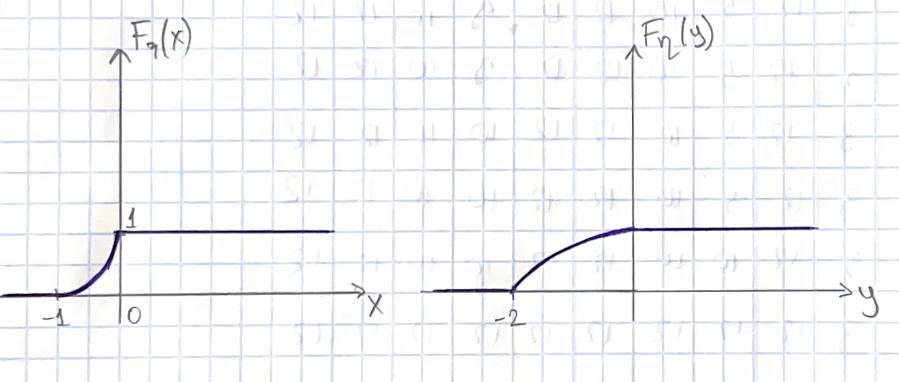
\includegraphics[width=0.5\linewidth]{2.jpeg}
    \caption{}
    \label{fig:enter-label}
\end{figure}
\end{proof}

%%%%%%%%%%%%%% ЗАДАНИЕ №2 %%%%%%%%%%%%%%
%% Условие задания №2
\begin{problem}
Найти распределения случайных величин $\zeta$ и $\nu$. Вычислить $\Expect\zeta$, $\Variance\zeta$, $\Expect\nu$ и $\Variance\nu$. Построить графики функций распределений $F_{\zeta}(z)$ и $F_{\nu}(n)$.
\end{problem}

%% Решение задания №2
\begin{proof}
$\zeta = 3\xi^4 + 2$. $\supp\xi = [-1;0]$, $\supp\zeta = [2;5]$. $g(\xi) = 3\xi^4 + 2$ и $g(\xi)$ монотонно убывает на $\supp\xi$. Тогда:
\begin{gather*}
g^{-1}(z) = -\sqrt[4]{\frac{z - 2}{3}}\\
(g^{-1}(z))' = \frac{-1}{4\sqrt[4]{3(z - 2)^3}}\\
\end{gather*}
Итого:
\[
p_{\zeta}(z) = \begin{cases}
    \frac{1}{2\sqrt[4]{3(z - 2)^3}}\cdot\left(1 - \sqrt[4]{\frac{z - 2}{3}}\right), & z \in [2;5]\\
    0, & \text{в отс. сл.}
    \end{cases}
\]
Считаем мат.ожидание и дисперсию:
\begin{gather*}
    \Expect\zeta = \int_{-\infty}^{\infty}z\cdot p_{\zeta}(z)dz = \int_{2}^{5}z\cdot p_{\zeta}(z)dz = \frac{11}{5} = 2.2\\
    \Expect\zeta^2 = \int_{-\infty}^{\infty}z^2\cdot p_{\zeta}(z)dz = \int_{2}^{5}z^2\cdot p_{\zeta}(z)dz = 5\\
    \Variance\zeta = \Expect\zeta^2 - \left(\Expect\zeta\right)^2 = 5 - 4.84 = 0.16
\end{gather*}
Функция распределения (график на рис. 3):
\[
F_{\zeta}(z) = \int\limits_{-\infty}^{z}p_{\zeta}(t)dt = \begin{cases}
    0, & z\in (-\infty;2]\\
    2\sqrt[4]{\frac{z - 2}{3}} - \sqrt{\frac{z - 2}{3}}, & z\in (2; 5]\\
    1, & z\in (5;\infty)
\end{cases}
\]
\begin{figure}[h!]
    \centering
    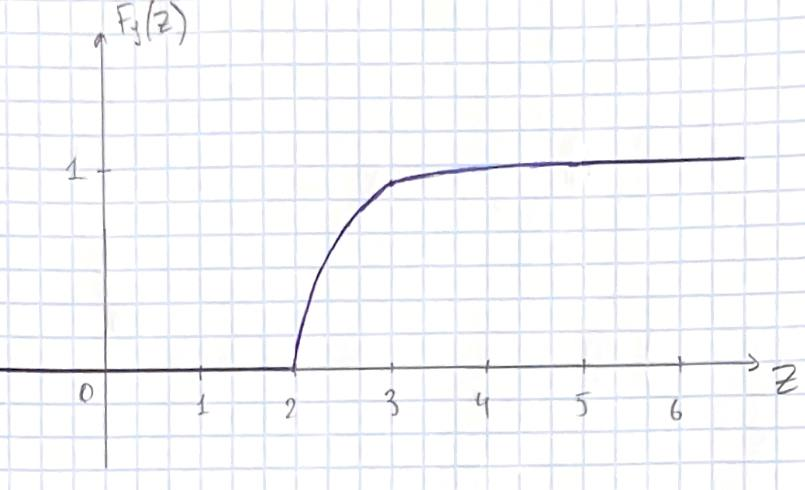
\includegraphics[width=0.5\linewidth]{3.jpeg}
    \caption{}
    \label{fig:enter-label}
\end{figure}
$\nu = \lfloor5\eta\rfloor$. $\supp\eta = [-2;0]$, $\supp\nu = \{-10, -9, -8, -7, -6, -5, -4, -3, -2, -1, 0\}$.
\[
\Prob(\nu = k) = \Prob(\eta\in[k/5; (k + 1)/5)) = -\int_{\frac{k}{5}}^{\frac{k + 1}{5}}\frac{y}{2}dy = \frac{-2k + 1}{100}
\]
Помимо этого учитываем, что для $\nu = 0$ $\eta = 0$, а значит $\Prob(\nu = 0) = 0$.\\
Строим таблицу:\\
\begin{table}[h!]
    \centering
    \begin{tabular}{|c|c|c|c|c|c|c|c|c|c|c|c|c|}
    \hline
        $\nu$ & -10 & -9 & -8 & -7 & -6 & -5 & -4 & -3 & -2 & -1 & 0 & $\sum$\\
    \hline
        $p_i$ & 0.19 & 0.17 & 0.15 & 0.13 & 0.11 & 0.09 & 0.07 & 0.05 & 0.03 & 0.01 & 0 & 1\\
    \hline
    \end{tabular}
\end{table}

Теперь считаем мат.ожидание и дисперсию:
\begin{gather*}
    \Expect\nu = \sum_{i: p_i > 0}a_ip_i = -7.15\\
    \Expect\nu^2 = \sum_{i: p_i > 0}a_i^2p_i = 56.65\\
    \Variance\nu = \Expect\nu^2 - \left(\Expect\nu\right)^2 = 56.65 - 51.1225 = 5.5275
\end{gather*}
Функция распределения (график на рис. 4):
\[
F_{\nu}(n) = \begin{cases}
    0, & n\in (-\infty;-10]\\
    0.19, & n\in (-10;-9]\\
    0.36, & n\in (-9;-8]\\
    0.51, & n\in (-8;-7]\\
    0.64, & n\in (-7;-6]\\
    0.75, & n\in (-6;-5]\\
    0.84, & n\in (-5;-4]\\
    0.91, & n\in (-4;-3]\\
    0.96, & n\in (-3;-2]\\
    0.99, & n\in (-2;-1]\\
    1, & n\in (-1;\infty)
\end{cases}
\]
\begin{figure}[h!]
    \centering
    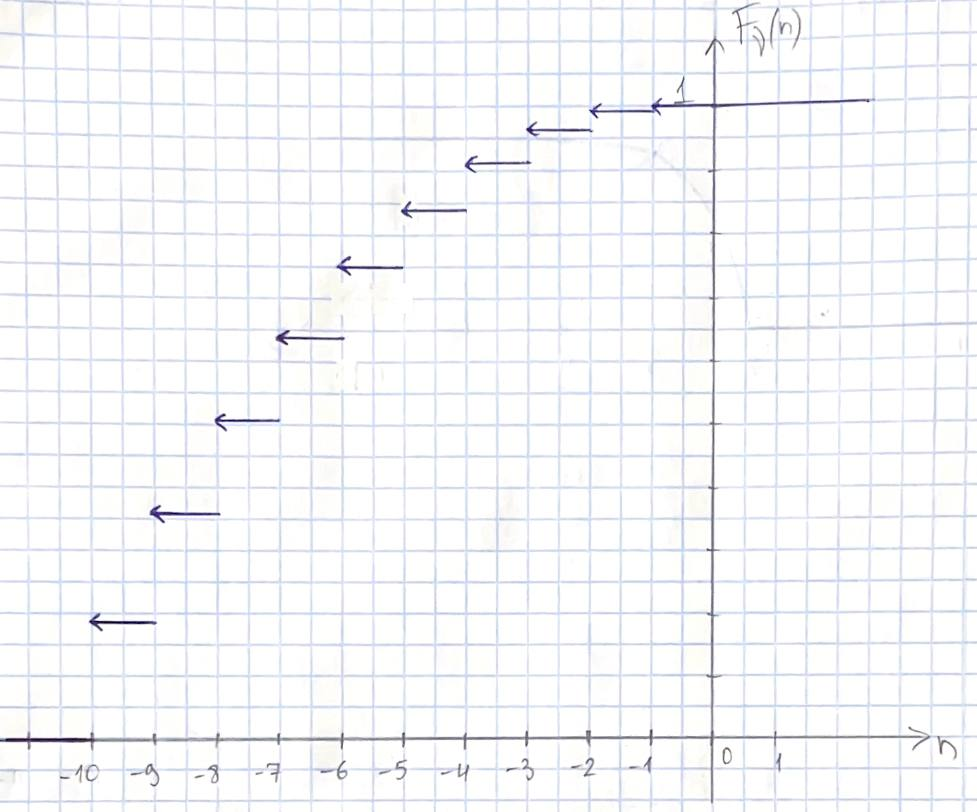
\includegraphics[width=0.5\linewidth]{4.jpeg}
    \caption{}
    \label{fig:enter-label}
\end{figure}
\end{proof}

%%%%%%%%%%%%%% ЗАДАНИЕ №3 %%%%%%%%%%%%%%
%% Условие задания №3
\begin{problem}
Вычислить вектор математических ожиданий, построить ковариационную и кореляционную матрицы для вектора $(\xi,\eta)$. Найти условное распределение $\xi$ при условии $\eta$. Вычислить $\Expect(\xi | \eta)$ и $\Variance(\xi | \eta)$.
\end{problem}

%% Решение задания №3
\begin{proof}
Мат.ожидание и дисперсия для $\xi$:
\begin{gather*}
    \Expect\xi = \int_{-\infty}^{\infty}x\cdot p_{\xi}(x)dx = \int_{-1}^{0}x\cdot(2x + 2)dx = -\frac{1}{3}\\
    \Expect\xi^2 = \int_{-\infty}^{\infty}x^2\cdot p_{\xi}(x)dx = \int_{-1}^{0}x^2\cdot(2x + 2)dx = \frac{1}{6}\\
    \Variance\xi = \Expect\xi^2 - \left(\Expect\xi\right)^2 = \frac{1}{6} - \frac{1}{9} = \frac{1}{18}
\end{gather*}
Мат.ожидание и дисперсия для $\eta$:
\begin{gather*}
    \Expect\eta = \int_{-\infty}^{\infty}y\cdot p_{\eta}(y)dy = \int_{-2}^{0}y\cdot\frac{-y}{2}dy = -\frac{4}{3}\\
    \Expect\eta^2 = \int_{-\infty}^{\infty}y^2\cdot p_{\eta}(y)dy = \int_{-2}^{0}y^2\cdot\frac{-y}{2}dy = 2\\
    \Variance\eta = \Expect\eta^2 - \left(\Expect\eta\right)^2 = 2 - \frac{16}{9} = \frac{2}{9}
\end{gather*}
Вектор мат.ожиданий:\\
\[
\Expect\begin{pmatrix} \xi \\ \eta \end{pmatrix} = \begin{pmatrix} -1/3 \\ -4/3 \end{pmatrix}
\]
Посчитаем ковариацию и корреляцию $\xi$ и $\eta$:
\begin{gather*}
\Expect\xi\eta = \iint_{\Real^2}xy\cdot p_{\xi,\eta}(x,y)dxdy = \int_{-1}^{0}dx\int_{-2}^{2x}xydy = \frac{1}{2}\\
\cov(\xi, \eta) = \Expect\xi\eta - \Expect\xi\cdot\Expect\eta = \frac{1}{2} = \frac{4}{9} = \frac{1}{18}\\
\rho(\xi,\eta) = \frac{\cov(\xi,\eta)}{\sqrt{\Variance\xi}\sqrt{\Variance\eta}} = \frac{1}{2}
\end{gather*}
Итого:
\[
\sum = \begin{pmatrix}
\frac{1}{18} & \frac{1}{18} \\
\frac{1}{18} & \frac{2}{9}
\end{pmatrix}
\]
\[
R = \begin{pmatrix}
1 & \frac{1}{2} \\
\frac{1}{2} & 1
\end{pmatrix}
\]
Найдем условное распределение $\xi$ при условии $\eta$:
\begin{gather*}
    p_{\xi|\eta=y_0} = \frac{p_{\xi,\eta}(x,y_0)}{p_{\eta}(y_0)} \text{ при } p_{\eta}(y) > 0\Rightarrow\\
    \Rightarrow p_{\xi|\eta=y_0} = \begin{cases}
        -\frac{2}{y_0}, & x\in [y_0/2; 0]\\
        0, & \text{в отс. сл.}
    \end{cases} \Rightarrow\\
    \Rightarrow p_{\xi|\eta} = \begin{cases}
        -\frac{2}{\eta}, & x\in [\eta/2; 0]\\
        0, & \text{в отс. сл.}
    \end{cases}
\end{gather*}
Условное мат.ожидание и условная дисперсия:
\begin{gather*}
    \Expect(\xi|\eta) = \int_{-\infty}^{\infty}x\cdot p_{\xi|\eta}(x)dx = \int_{\eta/2}^{0}x\cdot p_{\xi|\eta}(x)dx = \frac{\eta}{4}\\
    \Expect(\xi^2|\eta) = \int_{-\infty}^{\infty}x^2\cdot p_{\xi|\eta}(x)dx = \int_{\eta/2}^{0}x^2\cdot p_{\xi|\eta}(x)dx =\frac{\eta^2}{12}\\
    \Variance(\xi|\eta) = \Expect(\xi^2|\eta) - \left(\Expect(\xi|\eta)\right)^2 = \frac{\eta^2}{48}
\end{gather*}
Проверим свойство $\Expect(\Expect(\xi|\eta)) = \Expect\xi$:
\[
\Expect(\Expect(\xi|\eta)) = \Expect\left(\frac{\eta}{4}\right) = \frac{1}{4}\cdot\frac{-4}{3} = -\frac{1}{3} = \Expect\xi - \text{верно}
\]
Проверим свойство $\Expect(\Variance(\xi|\eta)) + \Variance(\Expect(\xi|\eta)) = \Variance\xi$:
\[
\Expect(\Variance(\xi|\eta)) + \Variance(\Expect(\xi|\eta)) = \Expect\left(\frac{\eta^2}{48}\right) + \Variance\left(\frac{\eta}{4}\right) = \frac{1}{24} + \frac{1}{72} = \frac{1}{18} = \Variance\xi - \text{верно}
\]
\end{proof}

%%%%%%%%%%%%%% ЗАДАНИЕ №4 %%%%%%%%%%%%%%
%% Условие задания №4
\begin{problem}
Найти распределение $\mu$. Вычислить $\Expect\mu$ и $\Variance\mu$. Построить график функции распределения $F_{\mu}(m)$.
\end{problem}

%% Решение задания №4
\begin{proof}
\begin{figure}[h!]
    \centering
    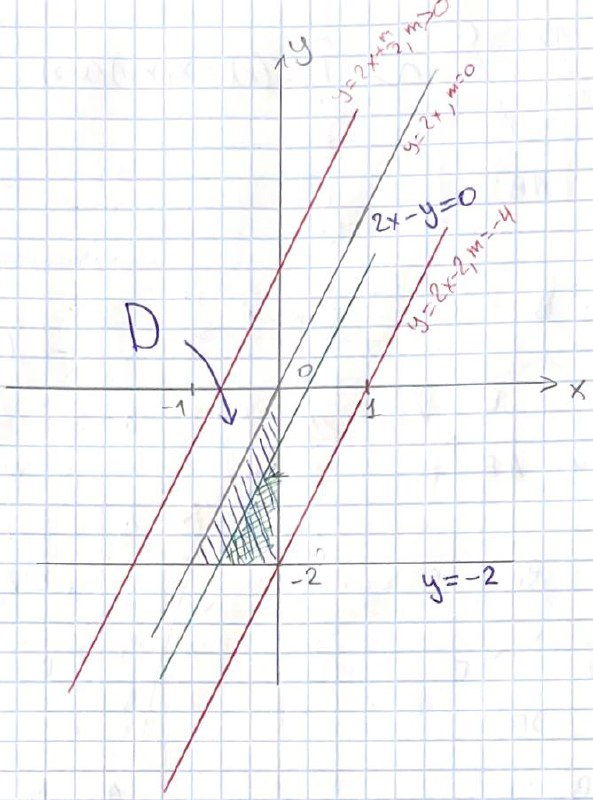
\includegraphics[width=0.5\linewidth]{5.jpeg}
    \caption{}
    \label{fig:enter-label}
\end{figure}
$\mu = -4\xi + 2\eta$. $F_{\mu}(m) = \Prob(\mu \le m) = \Prob(-4\xi + 2\eta\le m)$.\\
См. рис. 5. Из него слудует, что: 
\[
F_{\mu}(m) = \begin{cases}
    0, & m\in (-\infty;-4]\\
    \frac{(m + 4)^2}{16}& m\in (-4; 0]\\
    1, & m\in (0; \infty)
\end{cases}
\]
Зная функцию распределения находим плотность:
\[
p_{\mu}(m) = \begin{cases}
    \frac{m + 4}{8}& m\in [-4; 0]\\
    0, & \text{в отс. сл.}
\end{cases}
\]
Мат.ожидание и дисперсия:
\begin{gather*}
    \Expect\mu = \int_{-\infty}^{\infty}m\cdot p_{\mu}(m)dm = \int_{-4}^{0}m\cdot p_{\mu}(m)dm = -\frac{4}{3}\\
    \Expect\mu^2 = \int_{-\infty}^{\infty}m^2\cdot p_{\mu}(m)dm = \int_{-4}^{0}m^2\cdot p_{\mu}(m)dm = \frac{8}{3}\\
    \Variance\mu = \Expect\mu^2 - \left(\Expect\mu\right)^2 = \frac{8}{3} - \frac{16}{9} = \frac{8}{9}
\end{gather*}
График функции распределения на рисунке 6.
\begin{figure}[h!]
    \centering
    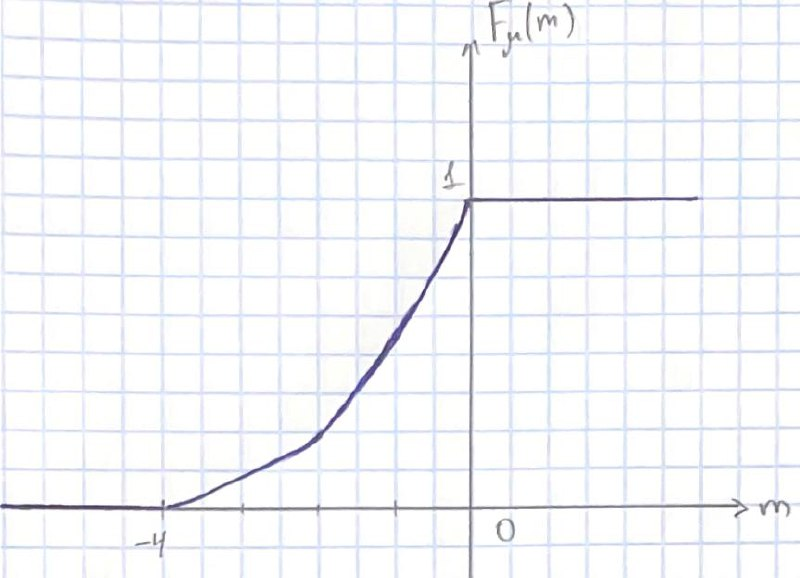
\includegraphics[width=0.5\linewidth]{6.jpeg}
    \caption{}
    \label{fig:enter-label}
\end{figure}
\end{proof}